\documentclass[notypeinfo,twoside,openright]{PostDocRep}
% \usepackage[utf8]{inputenc}  % xelatex 下不需要，原生支持 UTF-8
\usepackage{amsmath, amsthm, amssymb, booktabs, array, cases, graphicx, longtable,supertabular,multirow}
\usepackage{xcolor}
\usepackage{bookmark}
\usepackage{threeparttable}
\usepackage{subcaption} 
\usepackage{algorithm}
\usepackage{algpseudocode}
\usepackage{microtype}
\usepackage[super]{gbt7714}
\usepackage{placeins}
% \usepackage[T1]{fontenc}  % xelatex 下不需要，会导致字体冲突
\usepackage{fancyvrb} 

\newcolumntype{C}[1]{>{\centering\arraybackslash}m{#1}}
% 设置图形文件的搜索路径
\graphicspath{{chapter/}{figures/}}

% 取消链接的颜色
\hypersetup{colorlinks=false}

% 修改章的标题为英文格式
%\CTEXsetup[name={Chapter~,}, number={\arabic{chapter}}]{chapter}

% 小节标题靠左对齐
\ctexset{
  section = {
    format+={\flushleft}
  }
}

% 注意：在使用ctexbook的情况下，中文会自动使用宋体
% 配置代码块：确保下划线等特殊字符正常显示
\DefineVerbatimEnvironment{CodeBlock}{Verbatim}{%
    fontfamily=ptm,  % Times New Roman for English and numbers
    fontsize=\small,
    frame=single,
    framesep=2mm,
    baselinestretch=1.0,
    formatcom=\fontfamily{ptm}\selectfont,  % 确保使用Times New Roman
    codes={\catcode`\_=12\catcode`\&=12\catcode`\$=12\catcode`\#=12\catcode`\^=12\catcode`\~=12\catcode`\%=12},  % 将特殊字符设为普通字符（12表示普通字符）
}


\begin{document}


%%%%%%%%%%%%%%%%%%%%%%%%%%%%%%
%% 封面部分
%%%%%%%%%%%%%%%%%%%%%%%%%%%%%%

  % 中文封面内容
  % 请根据实际情况修改以下信息
  \classification{分类号示例}
  \confidential{公开}
  \UDC{UDC编号示例}
  \serialnumber{编号示例}
  \school{浙~江~大~学}
  \title[研究报告题目]{研究报告题目}
  \author{作者姓名}
  \workdate{20XX年X月}
  \submitdate{20XX年X月}
  \address{浙江大学（杭州）}
  \englishtitle{Research Report Title \\(English Title)}
  \major{流动站名称}
  \submajor{专业名称}
  \advisorent{企业导师姓名}
  \advisorschool{学校导师姓名}
  \institute{浙江大学XX学院}
  \begindate{20XX年X月X日}
  \ssdate{20XX年X月X日}

  % 封面、题名页
\maketitle


%%%%%%%%%%%%%%%%%%%%%%%%%%%%%%
%% 前言部分
%%%%%%%%%%%%%%%%%%%%%%%%%%%%%%
\frontmatter

  % 摘要
  \begin{abstract}
摘要部分用于简要介绍研究工作的主要内容、研究方法、主要结论和创新点。
摘要应独立成文，使读者能够快速了解报告的核心内容。

本示例模板展示博士后研究报告的摘要格式规范。摘要一般应包含以下几个方面：

（1）研究背景与意义：简要说明研究工作的背景、目的和意义。

（2）研究内容与方法：概述研究的主要内容、采用的研究方法和技术路线。

（3）主要结论与成果：总结研究的主要发现、结论和创新成果。

（4）应用价值与展望：说明研究成果的应用价值及未来研究方向。

摘要篇幅建议控制在500-1000字左右，内容应简明扼要、重点突出。
避免使用过于专业的术语，使摘要具有较强的可读性。

\keywords{关键词1，关键词2，关键词3，关键词4，关键词5}

\begin{englishabstract}
    The abstract section is used to briefly introduce the main content, 
    research methods, major conclusions, and innovations of the research work. 
    The abstract should be self-contained, enabling readers to quickly 
    understand the core content of the report.
    
    This template demonstrates the format requirements for the abstract 
    of a postdoctoral research report. The abstract generally should 
    include the following aspects:
    
    (1) Research background and significance: briefly explain the background, 
    purpose, and significance of the research work.
    
    (2) Research content and methods: outline the main research content, 
    research methods adopted, and technical approach.
    
    (3) Major conclusions and achievements: summarize the main findings, 
    conclusions, and innovative results of the research.
    
    (4) Application value and prospects: explain the application value 
    of research results and future research directions.
    
    The abstract length is recommended to be around 500-1000 words, 
    with concise and focused content. Avoid using overly specialized 
    terminology to ensure readability.
    
    \englishkeywords{Keyword 1, Keyword 2, Keyword 3, Keyword 4, Keyword 5}
\end{englishabstract}
\end{abstract}

  % 目录
  \pagenumbering{Roman} % 使用罗马数字
  \fancyfoot[C]{\thepage}
  \tableofcontents
  \newpage
  % 表格目录
  \listoftables
  % 插图目录
  \listoffigures


%%%%%%%%%%%%%%%%%%%%%%%%%%%%%%
%% 正文部分
%%%%%%%%%%%%%%%%%%%%%%%%%%%%%%
\mainmatter

\chapter{引言（示例章节）}
\label{chap:introduction}

本章介绍研究报告的基本结构和研究背景的撰写方法。

\section{研究背景}
研究背景部分应当说明研究工作的宏观背景和微观背景。
宏观背景可从行业发展趋势、国家政策导向等方面展开。
微观背景则应聚焦于具体研究领域的发展现状和存在问题。

例如，随着我国经济社会的快速发展，相关领域面临着一系列新的挑战和机遇。
这些挑战和机遇为本研究提供了重要的研究背景和研究动机\cite{example2023}。

\section{研究现状}
研究现状部分应当系统梳理国内外相关领域的研究进展。

\subsection{国外研究现状}
国外学者在该领域开展了大量研究工作。Smith等\cite{smith2022}提出了...
Johnson\cite{johnson2021}通过实验研究发现...

\subsection{国内研究现状}
国内学者也进行了相关研究。张三等\cite{zhang2020}研究了...
李四\cite{li2019}从理论角度分析了...

\subsection{研究现状总结}
综合国内外研究现状，可以发现：
（1）现有研究主要集中在...方面；
（2）在...方面的研究相对较少；
（3）存在...问题亟待解决。

\section{研究内容与目标}
\subsection{研究内容}
本报告主要研究内容包括：
\begin{enumerate}
    \item 第一项研究内容：简要说明研究内容的具体描述。
    \item 第二项研究内容：简要说明研究内容的具体描述。
    \item 第三项研究内容：简要说明研究内容的具体描述。
\end{enumerate}

\subsection{研究目标}
本研究的主要目标包括：
\begin{itemize}
    \item 目标一：简要描述研究目标。
    \item 目标二：简要描述研究目标。
    \item 目标三：简要描述研究目标。
\end{itemize}

\section{研究方法与技术路线}
本研究采用的主要研究方法包括理论分析、数值模拟和实验研究等。
技术路线如图\ref{fig:tech_route}所示。

\begin{figure}[htbp]
    \centering
    % 请替换为实际的流程图文件
    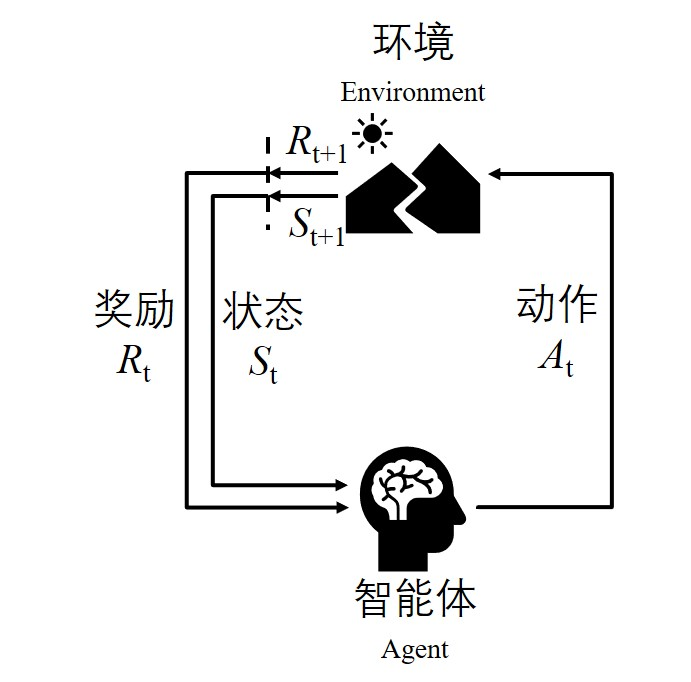
\includegraphics[width=0.8\textwidth]{figures/RL_Framework.jpg}
    \caption{研究技术路线示意图（示例）}
    \label{fig:tech_route}
\end{figure}

\section{报告结构安排}
本报告共分为六章，各章主要内容如下：

第一章为引言，介绍研究背景、研究现状和研究内容等。

第二章为研究方法示例章，展示图表、公式、算法等格式的使用方法。

第三章为实验研究示例章，展示表格、多图排版等格式的使用方法。

第四章为数值分析示例章，展示参考文献引用等格式的使用方法。

第五章为结果讨论示例章，展示结果展示格式。

第六章为结论与展望，总结研究成果并展望未来研究方向。
\chapter{研究方法示例章}
\label{chap:method}

本章展示研究报告中常用的格式元素，包括图表、公式、算法、代码块等。

\section{图的使用方法}
\subsection{单图插入}
图\ref{fig:single_figure}展示了单图插入的基本格式。
图片应当有清晰的图题，图号按章节编号。

\begin{figure}[htbp]
    \centering
    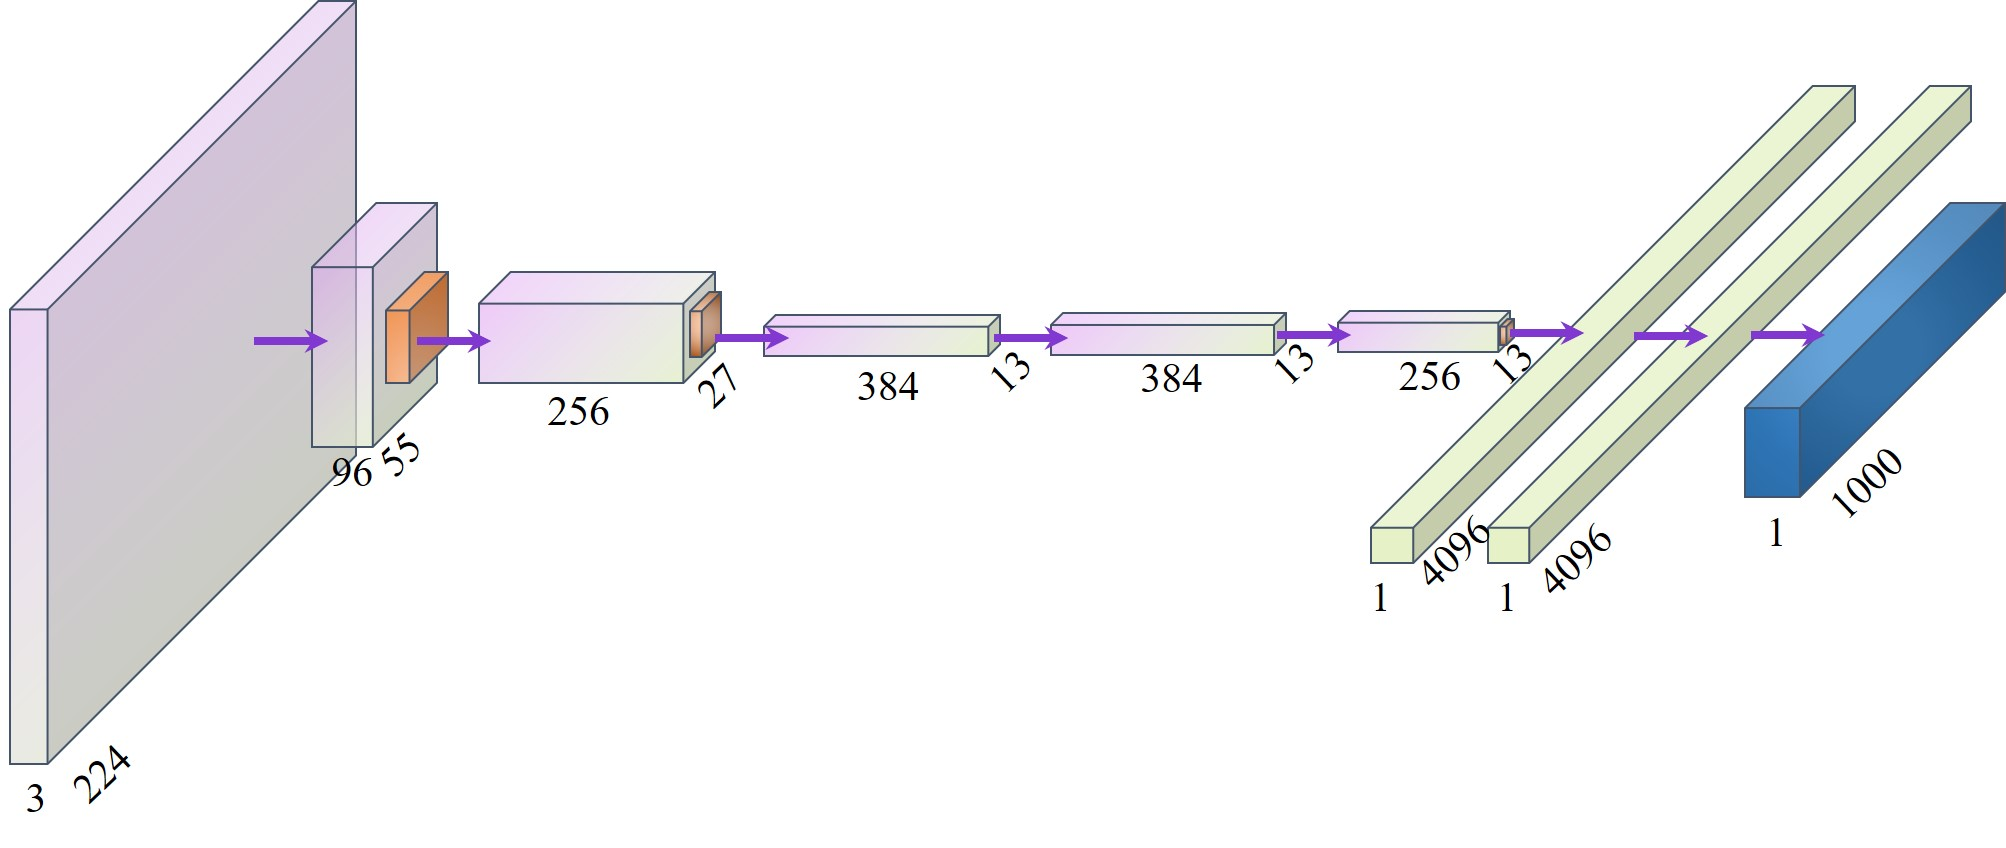
\includegraphics[width=0.5\textwidth]{figures/CNN.jpg}
    \caption{卷积神经网络结构示意图（单图示例）}
    \label{fig:single_figure}
\end{figure}

\subsection{多图并排}
当需要展示多张相关图片时，可采用并排排列的方式。
图\ref{fig:multi_figure}展示了多图并排的格式。

\begin{figure}[htbp]
    \centering
    \begin{subfigure}[b]{0.3\textwidth}
        \centering
        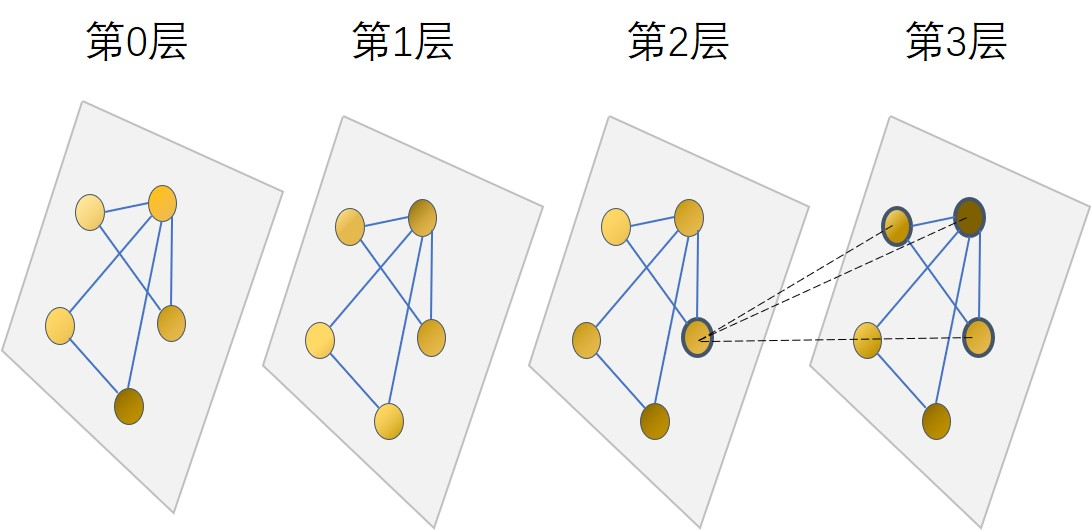
\includegraphics[width=\textwidth]{figures/GNN.jpg}
        \caption{图神经网络}
    \end{subfigure}
    \hfill
    \begin{subfigure}[b]{0.3\textwidth}
        \centering
        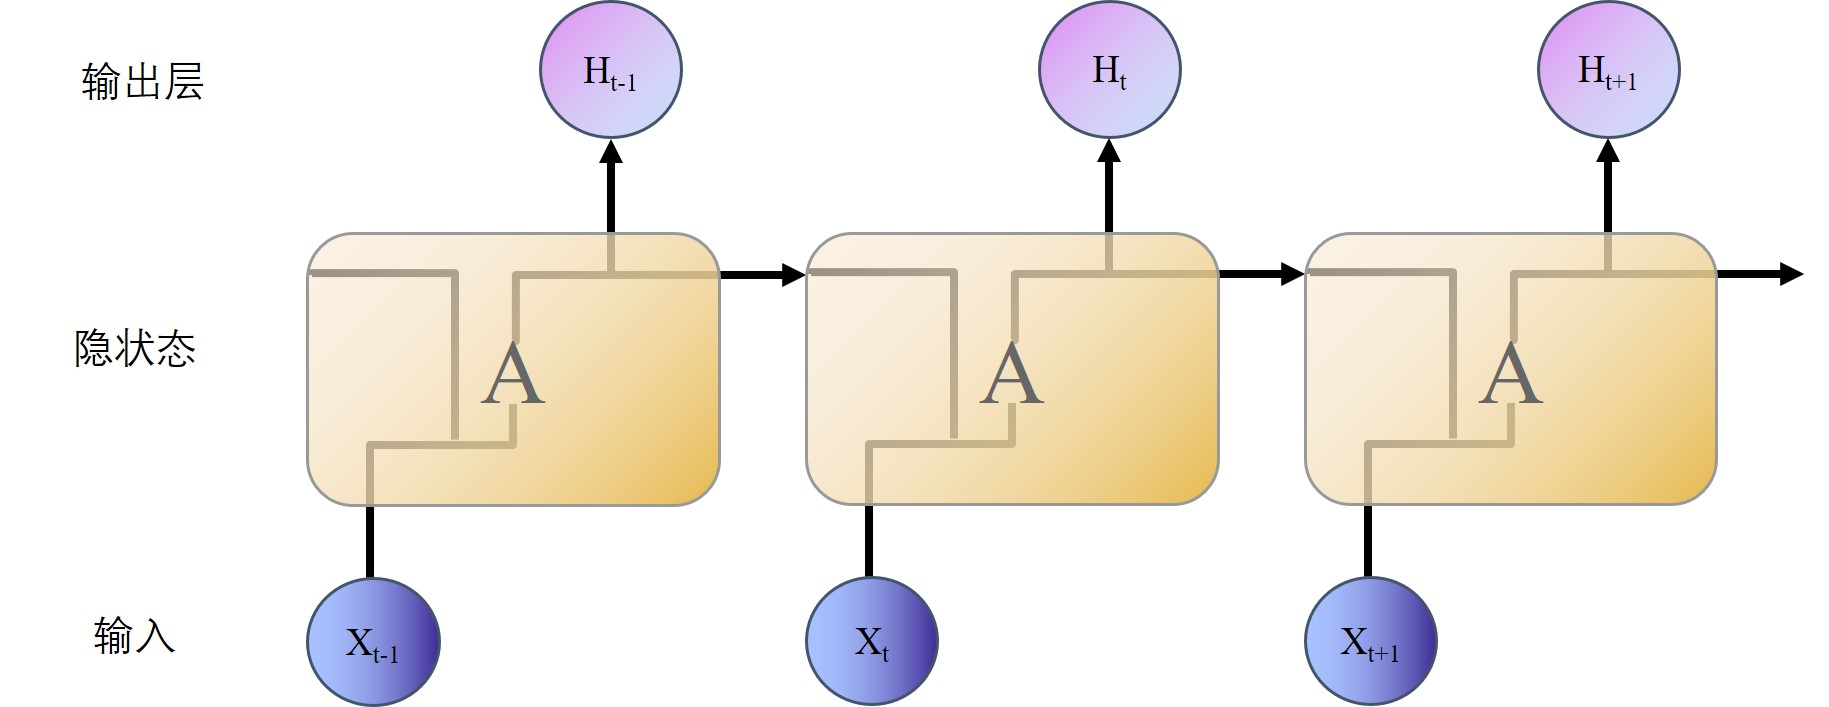
\includegraphics[width=\textwidth]{figures/RNN.jpg}
        \caption{循环神经网络}
    \end{subfigure}
    \hfill
    \begin{subfigure}[b]{0.3\textwidth}
        \centering
        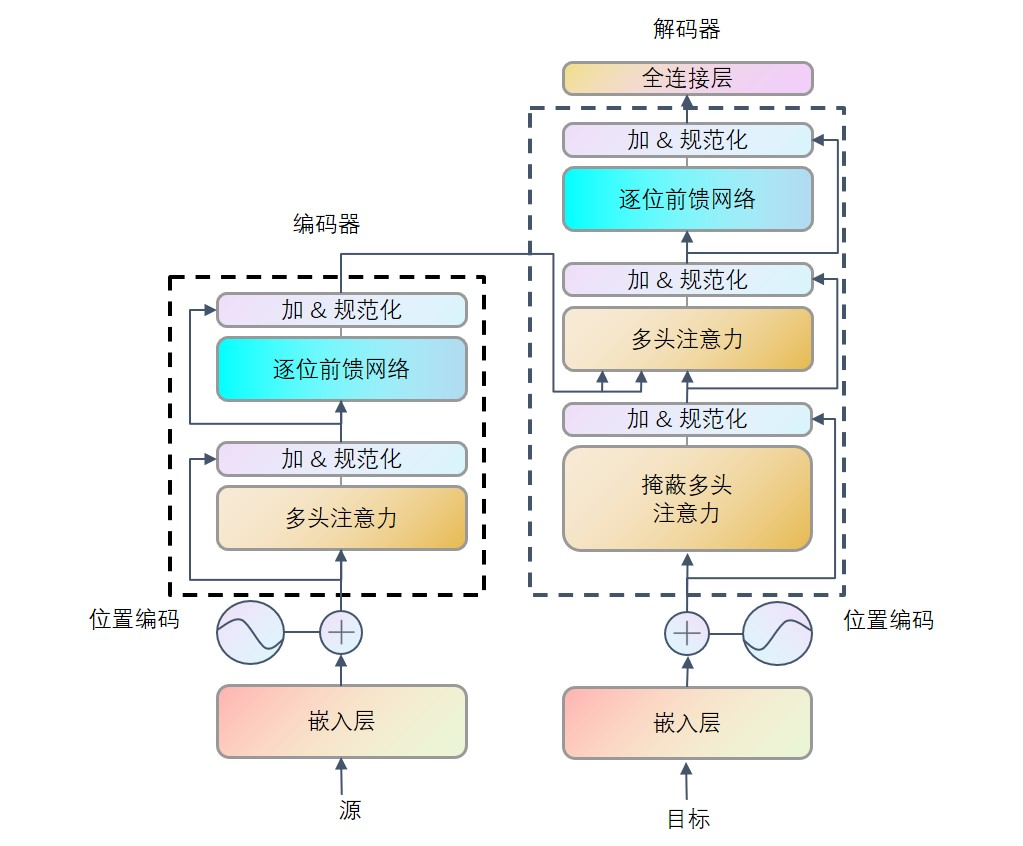
\includegraphics[width=\textwidth]{figures/Transformer.jpg}
        \caption{Transformer}
    \end{subfigure}
    \caption{不同类型神经网络结构示意图（多图并排示例）}
    \label{fig:multi_figure}
\end{figure}

\section{表格的使用方法}
\subsection{基本表格}
表\ref{tab:basic_table}展示了基本表格的格式。
表格应当有清晰的表题，表号按章节编号。

\begin{table}[htbp]
    \caption{基本表格示例}
    \label{tab:basic_table}
    \centering
    \begin{tabular}{lccc}
        \toprule
        参数名称 & 参数值1 & 参数值2 & 参数值3 \\
        \midrule
        参数A & 10 & 20 & 30 \\
        参数B & 40 & 50 & 60 \\
        参数C & 70 & 80 & 90 \\
        \bottomrule
    \end{tabular}
\end{table}

\subsection{三线表}
三线表是学术论文中常用的表格格式，只保留顶线、底线和栏目线。
表\ref{tab:three_line_table}展示了三线表的格式。

\begin{table}[htbp]
    \caption{三线表示例}
    \label{tab:three_line_table}
    \centering
    \begin{tabular}{lcc}
        \toprule
        实验编号 & 测量值1 & 测量值2 \\
        \midrule
        Exp-1 & 100.5 & 98.3 \\
        Exp-2 & 102.1 & 101.7 \\
        Exp-3 & 99.8 & 100.2 \\
        \bottomrule
    \end{tabular}
\end{table}

\subsection{复杂表格}
当表格内容复杂时，可采用合并单元格等方式。
表\ref{tab:complex_table}展示了复杂表格的格式。

\begin{table}[htbp]
    \caption{复杂表格示例（合并单元格）}
    \label{tab:complex_table}
    \centering
    \begin{tabular}{lcccc}
        \toprule
        \multirow{2}{*}{类别} & \multicolumn{2}{c}{指标A} & \multicolumn{2}{c}{指标B} \\
        \cmidrule(lr){2-3} \cmidrule(lr){4-5}
        & 值1 & 值2 & 值1 & 值2 \\
        \midrule
        类型1 & 50 & 60 & 70 & 80 \\
        类型2 & 55 & 65 & 75 & 85 \\
        类型3 & 60 & 70 & 80 & 90 \\
        \bottomrule
    \end{tabular}
\end{table}

\section{公式的使用方法}
\subsection{行内公式}
行内公式使用美元符号包裹，如 $E = mc^2$，$a^2 + b^2 = c^2$ 等。
行内公式适用于较短的数学表达式。

\subsection{独立公式}
独立公式使用equation环境，公式会自动编号。
公式\ref{eq:example}展示了独立公式的格式。

\begin{equation}
    y = f(x) = \frac{1}{n}\sum_{i=1}^{n} x_i^2
    \label{eq:example}
\end{equation}

\subsection{多行公式}
当公式较长需要分行时，可使用align环境。
公式\ref{eq:loss}和\ref{eq:gradient}公式展示了多行公式的格式。

\begin{align}
    L &= \sum_{i=1}^{n} \left( y_i - \hat{y}_i \right)^2 \label{eq:loss} \\
    \frac{\partial L}{\partial w} &= \sum_{i=1}^{n} 2\left( y_i - \hat{y}_i \right) \frac{\partial \hat{y}_i}{\partial w} \label{eq:gradient}
\end{align}

\subsection{矩阵公式}
矩阵可使用matrix环境表示。

\begin{equation}
    \mathbf{A} = \begin{bmatrix}
        a_{11} & a_{12} & a_{13} \\
        a_{21} & a_{22} & a_{23} \\
        a_{31} & a_{32} & a_{33}
    \end{bmatrix}
    \label{eq:matrix}
\end{equation}

\section{算法的使用方法}
算法可采用algorithm和algpseudocode环境。
算法\ref{alg:example}展示了算法的格式。

\begin{algorithm}[htbp]
    \caption{示例算法}
    \label{alg:example}
    \begin{algorithmic}[1]
        \Require 输入数据 $X$, 参数 $\theta$
        \Ensure 输出结果 $Y$
        \State 初始化参数 $\theta$
        \For{$i = 1$ to $N$}
            \State 计算中间结果 $z_i = f(x_i, \theta)$
            \If{$z_i > threshold$}
                \State 更新参数 $\theta$
            \EndIf
        \EndFor
        \State 返回结果 $Y$
    \end{algorithmic}
\end{algorithm}

\section{代码块的使用方法}
代码块可使用verbatim环境或自定义的CodeBlock环境。

\begin{CodeBlock}
def example_function(x, y):
    """示例函数"""
    result = x + y
    return result

# 调用示例
output = example_function(10, 20)
print(output)
\end{CodeBlock}

\section{定理与证明}
本模板支持定理、定义、引理等环境。

\begin{defn}[示例定义]
设 $f: \mathbb{R} \to \mathbb{R}$ 是一个函数，若对于任意 $x_1, x_2 \in \mathbb{R}$，
当 $x_1 < x_2$ 时有 $f(x_1) < f(x_2)$，则称 $f$ 为严格单调递增函数。
\end{defn}

\begin{thm}[示例定理]
设 $f$ 是连续函数，若 $f$ 在区间 $[a, b]$ 上严格单调递增，则 $f$ 在 $[a, b]$ 上有唯一最大值。
\end{thm}

\begin{proof}
证明过程略，请根据实际需要补充完整的证明。
\end{proof}
\chapter{实验研究示例章}
\label{chap:experiment}

本章展示实验研究部分的常见格式，包括实验设计、实验结果表格、实验数据图等。

\section{实验设计}
\subsection{实验目的}
本实验旨在验证相关理论分析的正确性，获取关键参数的实际数值。

\subsection{实验条件}
实验在标准实验室条件下进行，具体实验条件见表\ref{tab:experiment_conditions}。

\begin{table}[htbp]
    \caption{实验条件参数表}
    \label{tab:experiment_conditions}
    \centering
    \begin{tabular}{lll}
        \toprule
        参数类型 & 参数名称 & 参数值 \\
        \midrule
        环境参数 & 温度 & 25$\pm$2$^\circ$C \\
        环境参数 & 相对湿度 & 50$\pm$5\% \\
        设备参数 & 加载速率 & 1.0 mm/min \\
        设备参数 & 数据采集频率 & 100 Hz \\
        \bottomrule
    \end{tabular}
\end{table}

\subsection{试件信息}
本次实验共设计6个试件，试件基本信息见表\ref{tab:specimen_info}。

\begin{table}[htbp]
    \caption{试件基本信息表}
    \label{tab:specimen_info}
    \centering
    \begin{threeparttable}
    \begin{tabular}{C{2cm}C{3cm}C{3cm}C{3cm}}
        \toprule
        试件编号 & 尺寸参数(mm) & 材料类型 & 加载方式 \\
        \midrule
        Spec-1 & 200$\times$100$\times$10 & Type-A & 静态加载 \\
        Spec-2 & 200$\times$100$\times$10 & Type-A & 循环加载 \\
        Spec-3 & 300$\times$150$\times$15 & Type-B & 静态加载 \\
        Spec-4 & 300$\times$150$\times$15 & Type-B & 循环加载 \\
        Spec-5 & 400$\times$200$\times$20 & Type-C & 静态加载 \\
        Spec-6 & 400$\times$200$\times$20 & Type-C & 循环加载 \\
        \bottomrule
    \end{tabular}
    \begin{tablenotes}
        \footnotesize
        \item[*] 尺寸参数为试件的长度$\times$宽度$\times$厚度。
    \end{tablenotes}
    \end{threeparttable}
\end{table}

\section{实验结果}
\subsection{力学性能测试结果}
各试件的力学性能测试结果汇总于表\ref{tab:mechanical_results}。

\begin{table}[htbp]
    \caption{力学性能测试结果汇总表}
    \label{tab:mechanical_results}
    \centering
    \begin{tabular}{lcccc}
        \toprule
        试件编号 & 强度(MPa) & 延伸率(\%) & 弹性模量(GPa) & 破坏模式 \\
        \midrule
        Spec-1 & 350.5 & 12.3 & 210.0 & 拉断 \\
        Spec-2 & 340.2 & 15.1 & 205.5 & 疲劳 \\
        Spec-3 & 380.1 & 10.5 & 215.0 & 剪切 \\
        Spec-4 & 365.8 & 13.2 & 208.3 & 疲劳 \\
        Spec-5 & 420.3 & 8.5 & 220.0 & 弯曲 \\
        Spec-6 & 395.6 & 11.8 & 212.5 & 疲劳 \\
        \bottomrule
    \end{tabular}
\end{table}

\subsection{荷载-位移曲线}
荷载-位移曲线是实验结果的重要表现形式。
图\ref{fig:load_disp_curves}展示了荷载-位移曲线图的排版格式示例。
（注：此处使用神经网络图片作为格式占位示例，实际使用时请替换为真实的荷载-位移曲线图）

\begin{figure}[htbp]
    \centering
    \begin{subfigure}[b]{0.45\textwidth}
        \centering
        % 占位图片示例，请替换为实际的荷载-位移曲线图
        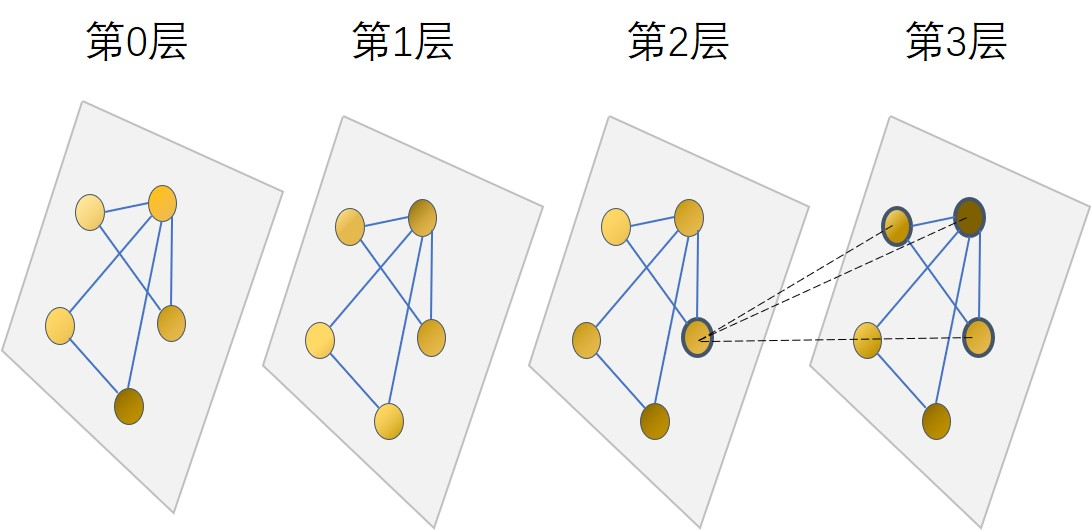
\includegraphics[width=\textwidth]{figures/GNN.jpg}
        \caption{静态加载试件（占位示例）}
    \end{subfigure}
    \hfill
    \begin{subfigure}[b]{0.45\textwidth}
        \centering
        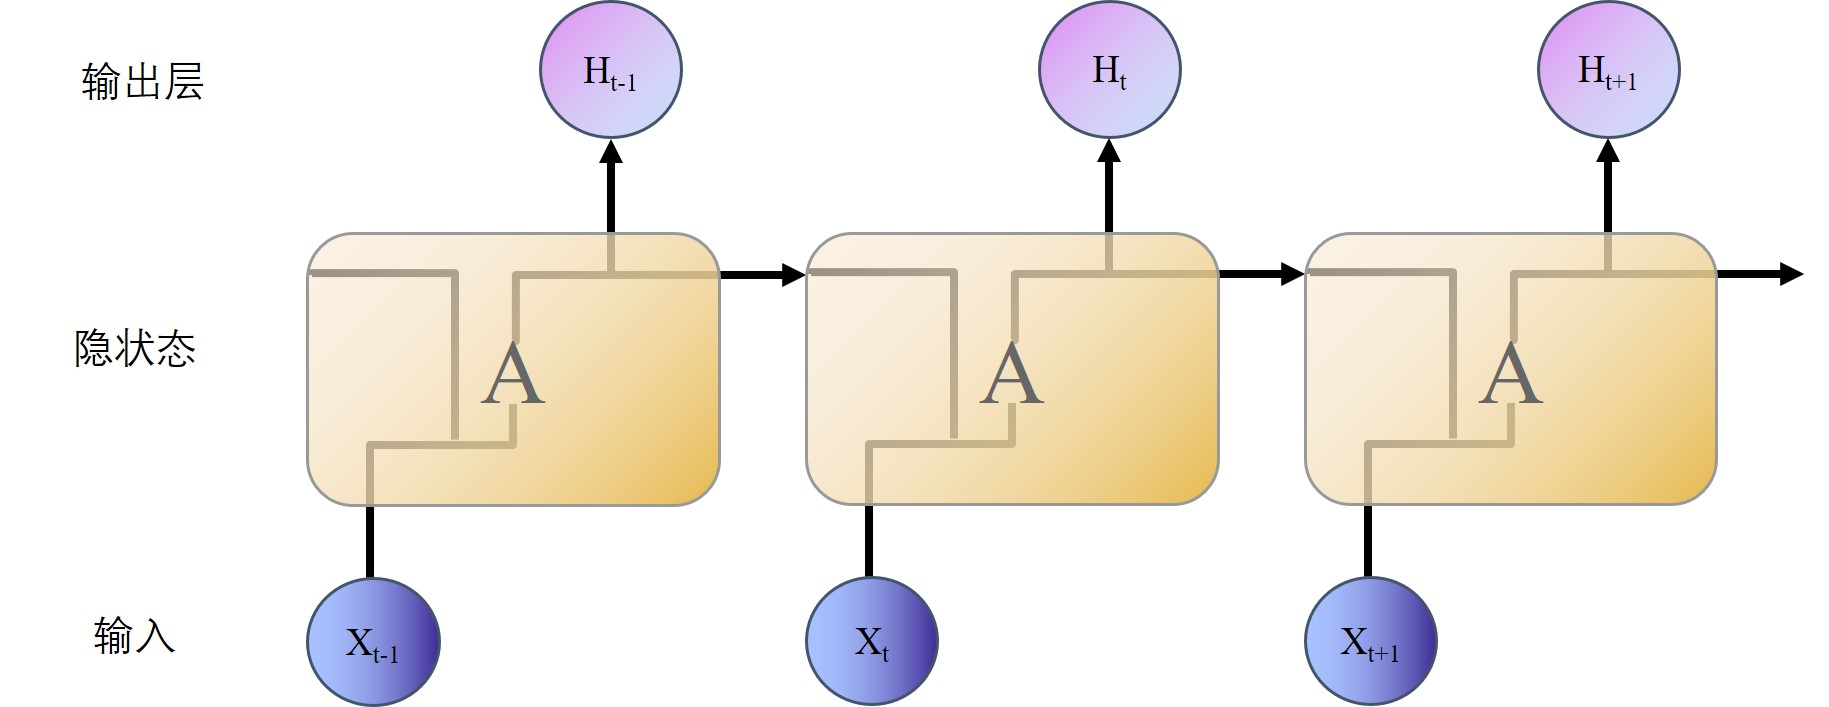
\includegraphics[width=\textwidth]{figures/RNN.jpg}
        \caption{循环加载试件（占位示例）}
    \end{subfigure}
    \caption{荷载-位移曲线排版格式示例（请替换为实际实验数据图）}
    \label{fig:load_disp_curves}
\end{figure}

\section{实验结果分析}
\subsection{强度分析}
从表\ref{tab:mechanical_results}可以看出，不同类型试件的强度存在明显差异。
Type-C试件强度最高，达到420.3 MPa，比Type-A试件高出约20\%。

\subsection{延伸率分析}
延伸率反映了材料的塑性变形能力。
循环加载试件的延伸率普遍高于静态加载试件。

\subsection{破坏模式分析}
不同加载方式下试件的破坏模式存在差异：
\begin{itemize}
    \item 静态加载试件主要表现为拉断、剪切或弯曲破坏；
    \item 循环加载试件主要表现为疲劳破坏。
\end{itemize}
\chapter{数值分析示例章}
\label{chap:analysis}

本章展示数值分析部分的常见格式，包括有限元模型、参数分析、参考文献引用等。

\section{数值模型建立}
\subsection{模型概述}
本研究采用有限元方法建立数值分析模型。
模型采用商业有限元软件进行分析，模型几何参数见表\ref{tab:model_params}。

\begin{table}[htbp]
    \caption{有限元模型参数表}
    \label{tab:model_params}
    \centering
    \begin{tabular}{lll}
        \toprule
        参数类别 & 参数名称 & 参数值 \\
        \midrule
        几何参数 & 模型尺寸 & 500$\times$300$\times$50 mm \\
        几何参数 & 单元尺寸 & 5 mm \\
        材料参数 & 弹性模量 & 210 GPa \\
        材料参数 & 泊松比 & 0.3 \\
        边界参数 & 底部约束 & 固定约束 \\
        边界参数 & 加载方式 & 位移控制 \\
        \bottomrule
    \end{tabular}
\end{table}

\subsection{材料模型}
材料本构模型是数值分析的关键。
本研究采用弹塑性材料模型，屈服准则采用von Mises准则\cite{vonmises1913}。

材料的应力-应变关系可表示为：
\begin{equation}
    \sigma = \begin{cases}
        E\varepsilon & \varepsilon \leq \varepsilon_y \\
        \sigma_y + H(\varepsilon - \varepsilon_y) & \varepsilon > \varepsilon_y
    \end{cases}
    \label{eq:stress_strain}
\end{equation}
式中，$E$为弹性模量，$\sigma_y$为屈服应力，$H$为硬化模量。

\section{扩散模型分析}
\subsection{扩散模型原理}
扩散模型是近年来深度学习领域的重要进展，广泛应用于图像生成、数据增强等任务。
图\ref{fig:model_validation}展示了扩散模型的基本架构和生成过程。

\begin{figure}[htbp]
    \centering
    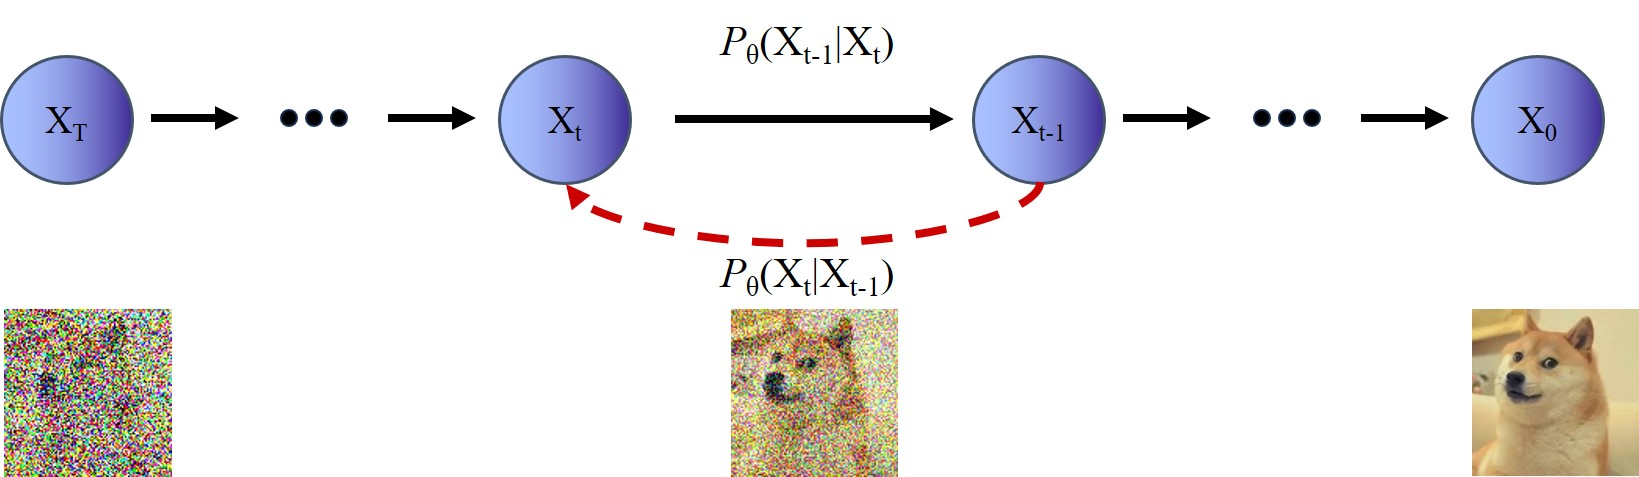
\includegraphics[width=0.8\textwidth]{figures/Diffusion.jpg}
    \caption{扩散模型架构与生成过程示意}
    \label{fig:model_validation}
\end{figure}

从对比结果可以看出，数值模型能够较好地模拟试验结果，误差控制在5\%以内\cite{validation2022}。

\section{参数分析}
\subsection{参数选择}
参数分析选取了以下关键参数进行研究：
\begin{enumerate}
    \item 几何参数：尺寸比例、厚度变化等；
    \item 材料参数：弹性模量、屈服强度等；
    \item 边界参数：约束方式、加载速率等。
\end{enumerate}

\subsection{参数分析结果}
参数分析结果汇总于表\ref{tab:param_analysis}。

\begin{table}[htbp]
    \caption{参数分析结果汇总表}
    \label{tab:param_analysis}
    \centering
    \begin{tabular}{lcccl}
        \toprule
        参数名称 & 基准值 & 变化范围 & 响应变化 & 影响程度 \\
        \midrule
        弹性模量 & 210 GPa & 180-250 & $\pm$15\% & 中等 \\
        屈服强度 & 350 MPa & 280-420 & $\pm$20\% & 显著 \\
        单元尺寸 & 5 mm & 2-10 & $\pm$8\% & 较小 \\
        加载速率 & 1.0 & 0.5-2.0 & $\pm$3\% & 较小 \\
        \bottomrule
    \end{tabular}
\end{table}

\section{参考文献引用格式}
\subsection{期刊论文引用}
期刊论文引用应注明作者、年份、期刊名称、卷号和页码\cite{smith2022,zhang2020}。

\subsection{书籍引用}
书籍引用应注明作者、书名、出版社和出版年份\cite{book2021}。

\subsection{学位论文引用}
学位论文引用应注明作者、论文题目、学校、年份\cite{thesis2020}。

\subsection{会议论文引用}
会议论文引用应注明作者、会议名称、年份、页码\cite{conference2023}。

\subsection{规范标准引用}
规范标准引用应注明标准编号和名称\cite{standard2018}。

正确引用参考文献是学术规范的重要组成部分。
\chapter{结果讨论示例章}
\label{chap:discussion}

本章展示结果讨论部分的常见格式，包括结果对比、机理分析、工程应用建议等。

\section{结果对比分析}
\subsection{不同方法对比}
本研究结果与已有研究成果的对比见表\ref{tab:result_comparison}。

\begin{table}[htbp]
    \caption{本研究结果与已有成果对比}
    \label{tab:result_comparison}
    \centering
    \begin{tabular}{lcccc}
        \toprule
        研究来源 & 方法类型 & 主要参数 & 结果数值 & 相对误差 \\
        \midrule
        本研究 & 数值模拟 & $E=210$ GPa & 385.6 MPa & --- \\
        文献\cite{smith2022} & 试验研究 & $E=205$ GPa & 380.2 MPa & 1.4\% \\
        文献\cite{zhang2020} & 理论分析 & $E=210$ GPa & 392.5 MPa & 1.8\% \\
        \bottomrule
    \end{tabular}
\end{table}

从对比结果可以看出，本研究结果与已有研究成果吻合良好，验证了研究方法的可靠性。

\subsection{误差分析}
误差来源主要包括以下几个方面：
\begin{enumerate}
    \item 数值离散化误差：有限元网格尺寸引入的离散化误差；
    \item 材料参数误差：材料本构参数与实际值存在偏差；
    \item 边界条件误差：简化边界条件与实际工况的差异。
\end{enumerate}

\section{机理分析}
\subsection{力学机理}
通过数值分析和试验验证，揭示了以下力学机理：

（1）荷载传递机理：荷载通过材料内部传递，应力分布呈现明显的不均匀性。

（2）变形机理：材料变形包括弹性变形和塑性变形两个阶段，塑性变形集中于高应力区域。

（3）破坏机理：材料破坏起源于应力集中区域，裂纹扩展导致最终破坏。

\subsection{影响因素分析}
影响研究结果的关键因素包括：
\begin{itemize}
    \item 材料因素：材料的力学性能直接影响研究对象的响应特性。
    \item 几何因素：结构几何形状决定了应力分布和变形模式。
    \item 边界因素：边界条件对数值分析结果有显著影响。
\end{itemize}

\section{工程应用建议}
\subsection{设计建议}
基于研究结果，提出以下设计建议：
\begin{enumerate}
    \item 参数选择建议：建议设计参数控制在合理范围内。
    \item 尺寸优化建议：建议结构尺寸比例控制在特定范围内以提高效率。
    \item 材料选择建议：建议选用性能稳定的材料。
\end{enumerate}

\subsection{施工建议}
施工过程中应注意以下事项：
\begin{itemize}
    \item 控制施工误差，确保几何尺寸满足设计要求；
    \item 严格控制材料质量，确保材料性能达标；
    \item 施工顺序应按照设计方案执行。
\end{itemize}

\section{研究局限性}
本研究存在以下局限性：

（1）研究范围局限：本研究仅针对特定工况进行研究，其他工况需进一步验证。

（2）方法局限：数值分析方法存在一定的简化假设，可能影响结果的准确性。

（3）数据局限：试验数据有限，可能影响结论的普适性。
\chapter{结论与展望}
\section{主要结论}
本研究围绕示例研究课题开展了系统的研究工作，主要结论如下：

（1）研究方法验证：本研究提出的数值分析方法经过试验验证，能够准确模拟研究对象的关键力学性能，误差控制在5\%以内，表明研究方法具有较高的可靠性。

（2）参数影响规律：通过参数分析，揭示了各关键参数对研究结果的影响规律。屈服强度对结果影响最为显著，相对变化达到20\%；弹性模量影响中等，相对变化约15\%；几何参数影响相对较小。

（3）机理揭示：通过数值分析和试验验证，揭示了研究对象在不同工况下的力学机理，包括荷载传递机理、变形机理和破坏机理。

（4）工程应用价值：基于研究结果提出了设计建议和施工建议，为实际工程应用提供了参考依据。

\section{创新点}
本研究的创新点主要包括：
\begin{enumerate}
    \item 提出了一种新的数值分析方法，能够准确模拟研究对象的复杂力学行为。
    \item 系统揭示了关键参数对研究结果的影响规律，填补了相关研究空白。
    \item 提出了面向工程应用的设计建议，具有实际应用价值。
\end{enumerate}

\section{研究展望}
尽管本研究取得了一定成果，但仍有以下问题值得进一步研究：

（1）研究范围拓展：本研究仅针对特定工况进行研究，建议拓展研究范围，验证结论的普适性。

（2）方法改进：数值分析方法存在简化假设，建议进一步完善分析模型，提高结果的准确性。

（3）工程验证：建议开展更多的工程验证研究，检验研究成果在实际工程中的应用效果。

（4）新方法探索：建议探索新的研究方法，如机器学习方法等，提高研究效率。
% 致谢
\begin{thanks}

感谢流动站和合作导师提供的科研平台与指导。
导师在学术研究、论文撰写等方面给予了悉心指导和帮助，
为本研究的顺利完成奠定了坚实基础。

感谢所在单位和合作导师在科研项目、实验条件等方面给予的支持，
为本研究的开展创造了良好的研究环境。

感谢课题组成员在研究过程中给予的帮助和协作，
在讨论、试验、数据分析等环节共同攻克了诸多难题。

感谢家人对博士后工作的理解和支持，
为我顺利完成研究工作提供了重要保障。

最后，感谢各位评审专家对本报告提出的宝贵意见和建议。

\end{thanks}

% 参考文献
% 使用 BibTeX（gbt7714宏包已自动设置样式）
\bibliography{bib/tex}

% 附录
\appendix

% \include{chapter/chap-req}


%%%%%%%%%%%%%%%%%%%%%%%%%%%%%%
%% 附件部分
%%%%%%%%%%%%%%%%%%%%%%%%%%%%%%
\backmatter
% 发表文章目录
\begin{publications}{99}
  \pubsection{博士后期间发表的学术论文清单}
  \item 作者1, 作者2, 作者3. 论文标题示例[J]. 期刊名称示例, 20XX, 卷号(X): 页码.
  \item 作者1, 作者2, 作者3, 作者4. 论文标题示例二[J]. 期刊名称示例, 20XX, 卷号(X): 页码.
  \item 作者1, 作者2. 论文标题示例三[C]. 会议名称示例, 20XX: 页码.

  \pubsection{博士后期间申请的专利及软著}
  \item 发明专利, 作者1, 作者2, 作者3. 专利名称示例（专利号示例）
  \item 软件著作权, 作者1, 作者2. 软件名称示例V1.0, 登记号示例.
\end{publications}

% 个人简历
\begin{resume}

\begin{resumesection}{基本情况}
作者姓名，性别，籍贯，出生年月，
某某单位与某某大学联合培养博士后。
（请根据实际情况填写个人基本信息）

\end{resumesection}

\begin{resumelist}{教育状况}
20XX年X月至20XX年X月，某某大学，某某学院某某专业，博士。

20XX年X月至20XX年X月，某某大学，某某学院某某专业，硕士。

20XX年X月至20XX年X月，某某大学，某某学院某某专业，本科。
\end{resumelist}

\begin{resumelist}{工作经历}
20XX年X月至今，某某单位与某某大学联合培养博士后在站工作。

20XX年X月至20XX年X月，某某单位，从事某某工作。
\end{resumelist}

\begin{resumelist}{研究兴趣}
研究方向1，研究方向2，研究方向3。
（请根据实际情况填写研究兴趣）
\end{resumelist}

\begin{resumelist}{联系方式}
通讯地址：省市区街道门牌号

邮编：XXXXXX

E-mail: xxx@xxx.edu.cn
\end{resumelist}

\end{resume}



\end{document}